\input{report-header.tex}
\renewcommand{\clearpage}{}
\begin{document}

\section{Введение}
Существуют задачи, решение которых может быть сведено к решению СЛАУ большого размера с разреженной матрицей некоторого вида. К подобным задачам, например, относится поиск численного решения дифференциального уравнения или численный расчет параметров сложных электрических цепей. Для наиболее часто встречающихся видов матриц, таких как, трех- или пятидиагональных, блочно-диагональных, уже разработаны собственные оптимизации, позволяющие решить СЛАУ быстрее, чем за квадратичное время от числа неизвестных, вплоть до линейного. Однако в случае, если постановка задачи не может быть сведена математическими преобразованиями ни к одному из оптимальных с точки зрения вычислительной сложности решения видов, приходится или ограничиваться медленными классическими методами, не зависящими от структуры матрицы, или строить грубое начальное приближение исходной матрицы и приближать ее решение к искомому итерационными методами. Как правило, такое начальное приближение получается некоторыми структурными преобразованиями исходной матрицы, например занулением определенных областей в методе получения неполного LU разложения, что отражается на точности начального приближения решения СЛАУ. Предполагается, что использование методов, учитывающих качественные характеристики данных, содержащихся в матрице, может позволить построить более точную аппроксимацию исходной матрицы необходимого вида и таким образом уменьшить необходимое число итераций для получения искомого решения СЛАУ с заданной точностью.

\section{Методы решения СЛАУ}
В первую очередь, методы решения СЛАУ могут быть разделены на решающие СЛАУ общего и частного вида. Методы решения СЛАУ частного вида не рассматриваются в данной работе, т.к. уже имеют достаточное число методов решения, специфичных для каждого из случаев, в общем случае выполняющихся быстрее любого из общих методов решения СЛАУ. Очевидно, что методы решения СЛАУ частного вида не могут быть эффективно применены в задачах с матрицей, не приводимому к необходимому виду, что и составляет их основное ограничение. В свою очередь, методы решения СЛАУ общего вида как правило работают медленнее методов для решения СЛАУ частного вида, однако являются универсальными и по этой причине рассматриваются в этой работе.

Во-вторых, методы решения СЛАУ могут быть разделены на методы учитывающие и не учитывающие разреженность СЛАУ. Те методы, которые учитывают разреженность, позволяют находить эффективное с точки зрения используемой для хранения матрицы СЛАУ памяти в процессе вычисления решение. В свою очередь, методы не учитывающие разреженность, являются сложными в применении для СЛАУ большого размера, т.к. могут потребовать квадратичного объема памяти в зависимости от числа неизвестных.

Наконец, методы рещения СЛАУ могут быть разделены две основные группы -- прямые и итерационные. Прямые методы позволяют получить точное аналитическое решение однако как правило имеют высокую вычислительную сложность. Итерационные методы, в свою очередь, в некоторых случаях позволяют получить решение быстрее прямых методов, которое в большинстве случаев является лишь приближением точного решения СЛАУ с заданной точностью, а также могут иметь условную сходимость.

\subsection{Итерационные методы}
Основной идеей современных итерационных методов приближенного и точного решения СЛАУ является представление задачи поиска решения системы уравнений
\begin{equation*}
  \mathbf{A}\mathbf{x} = \mathbf{b}, \mathbf{A} \in \mathbb{C}_{n \times n},
 \end{equation*}
как минимума функции 
\begin{equation*}
  \Psi(\mathbf{x}) = \frac{1}{2}\mathbf{x}^H \mathbf{A} \mathbf{x} - \mathbf{b}^H \mathbf{x} + \gamma
\end{equation*}
на пространстве Крылова 
\begin{equation*}
  K_n(\mathbf{A}, \mathbf{v}) = span\left\{ \mathbf{v}, \mathbf{A}\mathbf{v}, ..., \mathbf{A}^{n-1}\mathbf{v} \right\}. 
\end{equation*}
Минимизация производится по методу градиентного спуска, где $\nabla\Psi(\mathbf{x}) = \mathbf{A}\mathbf{x} - \mathbf{b}$. В качестве крыловского пространства используется $K_n(\mathbf{A}, \mathbf{r}_0)$, где $\mathbf{r}_i = \mathbf{b} - \mathbf{A}\mathbf{x}_i, i \in [0, n-1]$, $\mathbf{x}_0$ - начальное приближение решения СЛАУ. Такой подход позволяет найти приближенное решение СЛАУ $\mathbf{x}_n \simeq \mathbf{x}^*$ как линейную комбинацию векторов линейной оболочки крыловского пространства, т.е. $\mathbf{x}_n \in \mathbf{x}_0 + K_n(\mathbf{A}, \mathbf{r}_0)$.


Основным различием итерационных методов решения СЛАУ является процесс построения $K_{i+1}(\mathbf{A}, \mathbf{r}_0)$, при котором $\mathbf{r}_{i+1}$ строится на основе выбора направления градиентного спуска(для семейства GC методов) или минимизации $\mathbf{A}$-нормы $\mathbf{x}_{i+1}$, где $||\mathbf{v}||_A = \sqrt{\mathbf{v}^H \mathbf{A} \mathbf{v}}$, для MinRES, GMRES.


Единственным итерационным методом, сходящимся к точному решению СЛАУ за не более чем $2n$ итераций является метод GMRES~\cite{krylovOverview}. Несмотря на реальную высокую скорость сходимости ($n_{real} \ll 2n$)~\cite{baseIDRs}, этот метод требует полного перестроения ортогонального базиса крыловского пространства на каждой итерации, что приводит к существенным затратам по времени выполнения и используемой памяти. Однако, вне зависимости от вычислительной сложности, этот метод может быть использован для оценки эффективности работы разрабатываемого метода по числу итераций.


Наиболее оптимальным с точки зрения числа требуемых итераций и вычислительных затрат на одну итерацию является метод IDR(s), в основе которого лежит выбор $\mathbf{r}_i$ таким образом, что $\mathbf{r}_i \in K_{i}, K_{j} \subseteq K_{j-1} \forall j \in [1, j]$. Благодаря такому выбору очередного вектора линейной оболочки, происходит понижение размерности крыловского пространства, реально необходимого для вычисления приближенного решения СЛАУ с заданной точностью. Алгоритм поиска решения по методу IDR(s) имеет вычислительную сложность порядка $O(n + \frac{n}{s})$~\cite{baseIDRs, advancedIDRs}, что выигрывает у прочих итерационных методов, в случае $s > 1$.


С точки зрения исследования, наиболее интересной задачей является предобуславливание матрицы для приведения ее виду, удобному для применения одного из итерационных методов. Выбор правильного предобуславливателя является залогом получения решения с заданной точностью за малое число итераций, а также получения наиболее точного начального приближения решения. Предобуславаливатели могут быть ``количественными'', т.е. такими, которые позволяют получить начальное приближение искомого вида засчет исключения части элементов из матрицы не основываясь при этом на самих данных, содержащихся в матрице, и ``качетсвенными'', т.е. такими, которые способны получить начальное приближение так же путем исключения некоторых элементов, но на основе анализа информации, содержащейся в матрице. Примерами количественных предобуславливателей являются неполное LU-разложение или получение верхнетреугольной матрицы путем отбрасывания элементов ниже главной диагонали, качетсвенные же предобуслаадиватели не так распространены, однако хорошим примером является SVD-разложение матрицы. Поиск качественного предобуславливателя, способного получить искомый вид матрицы за приемлемое (как минимум субквадратичное) время является одним из направлений исследования данной работы.


\subsection{Прямые методы}
Прямые методы имеют значительное преимущество над итерационными, т.к. в результате использования приводят к точному решению СЛАУ. Их недостатком является высокая вычислительная сложность для матриц общего вида, что приводит к росту научного интереса в области поиска оптимизаций решения СЛАУ с матрицами частного вида, часто встречающися в процессе решения конкретных прикладных задач, например, метод матричной прогонки для систем дифференциальных уравнений~\cite{progonka}. В общем случае, для эффективного решения СЛАУ прямыми методами, в настоящее время применяется метод разложения исходной матрицы в линейную комбинацию матриц определенного вида -- факторизация, с дальнейшим применением прямых методов, оптимизированных под каждый из присутвующих в разложении видов матриц для получения итогового решения СЛАУ. Среди наиболее популярных методов факторизации можно отметить такие, как LU-разложение~\cite{wikiLU}, QR-разложение~\cite{wikiQR}, разложение Холецкого~\cite{wikiCholesky}, иерархическое разложение~\cite{solverOverview, baseHSS} и другие.


Среди прямых методов решения больших разреженных СЛАУ наиболее оптимальной по вычислительной сложности и необходимой памяти является группа иерархических методов($\mathscr{H}$, $\mathscr{H}^2$, HSS~\cite{baseHSS, fastHSS, probHSS}).


\section{Методы факторизации матриц}
Для ускорения работы или попросту применения как прямых, так и итерационных методов в общем случае может понадобиться выполнение факторизации матрицы в линейную комбинацию матриц определенного вида. Далее будут описаны несколько наиболее популярных методов факторизации матриц -- иерархическое, сингулярное, QR, LU и другие разложения.

\subsubsection{Иерархическая факторизация}
 Основной идеей является представление исходной матрицы в виде бинарного дерева блоков(\reffig{hssTree}) некоторого фиксированного размера, каждый из которых может быть представлен линейной комбинацией своих потомков. Такой подход позволяет совместить эффективную схему хранения с хорошо параллелизуемой системой решения СЛАУ от листьев к корню, при которой для блоков на листьях выполняется быстрый алгоритм решения СЛАУ небольшого фиксированного размера, а для уровней выше достаточно выполнить свертку по известному рекуррентному соотношению, получаемому на этапе конструирования иерархического разложения(\reffig{hssFactor}).


\begin{figure}[h!]
	\centering
	\begin{minipage}{.45\textwidth}
		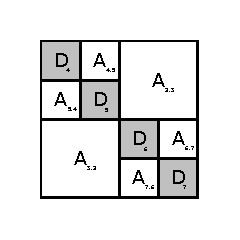
\includegraphics[width=.9\linewidth]{img/hssFactor.eps}
		\caption{Пример иерархической факторизации\label{hssFactor}}
	\end{minipage}
	\hfill
	\begin{minipage}{.45\textwidth}
		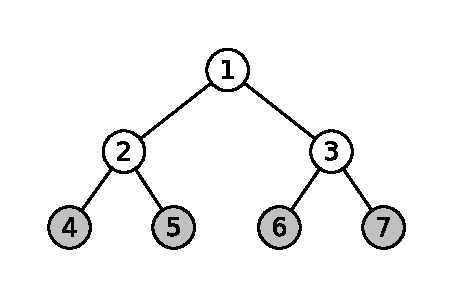
\includegraphics[width=.9\linewidth]{img/hssTree.eps}
		\caption{Дерево блоков иерархической факторизации\label{hssTree}}
	\end{minipage}
\end{figure}


Для того, чтобы матрица $\mathbf{A} \in \mathbb{C}_{N \times N}$, имеющая блочную тесселяцию из $K$ блоков, как показано на~\reffig{hssFactor}, являлась иерархически факторизуемой, т.е. представимой в виде бинарного дерева блоков $T$, как показано на~\reffig{hssTree}, необходимо чтобы выполнялись следующие условия:
\begin{itemize}
	\item Ранг каждого из внедиагональных блоков $\mathbf{A}_{i,j}$ не должен превышать $k$:
		\[
			rank\left(\mathbf{A}_{i,j}\right) \le k,~\forall i \ne j: 0 < i < K, 0 < j < K
		\]
	\item Для каждого из внедиагональных блоков, находящихся на одном уровне в дереве $T$, $\mathbf{A}_{i,j}$ существуют матрицы $\mathbf{U}, \mathbf{B}, \mathbf{V}$, такие, что матрица $\mathbf{A}_{i,j}$ может быть разложена по базису из $k$ векторов следующим образом:
		\[
        	\mathbf{A}_{i,j} = \mathbf{U}_{i} \mathbf{B}_{i,j} \mathbf{V}^*_{i},
		\]
		где $\mathbf{A} \in \mathbb{C}_{q \times q}, \mathbf{U}^{b}_{i}, \mathbf{V}^{b}_{i} \in \mathbb{C}_{q \times k}, \mathbf{B} \in \mathbb{C}{k \times k}$, причем, для каждого нелистового блока базисные матрицы $\mathbf{U}^{b}_{i}, \mathbf{V}$ могут быть рекуррентно выражены через аналогичные матрицы их наследников:
		\[
			\mathbf{U}^{b}_{i} =
			\begin{bmatrix}
				\mathbf{U}^{b}_{2i+1} & \mathbf{0} \\
				\mathbf{0} & \mathbf{U}^{b}_{2i+2} \\
			\end{bmatrix}
			\cdot
			\mathbf{U}_{i} 
		\]
\end{itemize}


Преимуществом иерархической факторизации является наличие алгоритма получения решения СЛАУ линейной от размера матрицы вычислительной сложности~\cite{baseHSS}. Основным недостатком является высокая сложность построения самого разложения, в худшем случае требующая $O(N^2)$~\cite{fastHSS} операций для матрицы $M_{N \times N}$, а в лучшем $O(k^2N)$~\cite{probHSS}, где $k$ - ранг блоков на листьях дерева.


\subsubsection{Примеры использования иерархического разложения}
Иерархическая факторизация матрицы $\mathbf{A} \in \mathbb{C}_{N \times N}$ может быть использована для быстрого вычисления произведения матрицы на вектор. Согласно~\cite{probHSS}, существует следующий алгоритм вычисления произведения матрицы на вектор $\mathbf{b} = \mathbf{A}\mathbf{x}$ линейной от размерности матрицы вычислительной сложности $O(kN)$:
\begin{enumerate}
	\item Для каждого листа $l$ вычисляется:
	\[
		\mathbf{x}^{\prime}_{l} = \mathbf{V}^{*}_{l} \mathbf{x}_{l};
	\]
	\item Для каждой нелистовой вершины $v$ дерева $T$ с потомками $l_1$ и $l_2$ от потомка к предку вычисляется:
	\[
		\mathbf{x}^{\prime}_{v} = \mathbf{V}^{*}_{v}
		\begin{bmatrix}
			\mathbf{x}^{\prime}_{l_1} \\
			\mathbf{x}^{\prime}_{l_2}
		\end{bmatrix};
	\]
	\item Для каждой нелистовой вершины $v$ дерева $T$ с потомками $l_1$ и $l_2$ от предка к потомку вычисляется:
	\[
		\begin{bmatrix}
			\mathbf{b}^{\prime}_{l_1} \\
			\mathbf{b}^{\prime}_{l_2}
		\end{bmatrix}
		=
		\begin{bmatrix}
			\mathbf{0} & \mathbf{B}_{l_1,l_2} \\
			\mathbf{B}_{l_1,l_2} & \mathbf{0}
		\end{bmatrix}
		\begin{bmatrix}
			\mathbf{x}^{\prime}_{l_1} \\
			\mathbf{x}^{\prime}_{l_2}
		\end{bmatrix}
		+ \mathbf{U}_{v}\mathbf{b}^{\prime}_{v};
	\]
	\item Наконец, для каждого листа $l$ вычисляются части итогового результата:
	\[
		\mathbf{b}_{l} = \mathbf{U}_{l}\mathbf{b}^{\prime}_{l} + \mathbf{D}_{l}\mathbf{x}_{l}.
	\]
\end{enumerate}

\subsection{Сингулярное разложение}
Сингулярное разложение -- это разложение прямоугольной матрицы $\mathbf{A}$ вида $\mathbf{A} = \mathbf{U} \mathbf{\Sigma} \mathbf{V}^*$, где $\mathbf{U}$ и $\mathbf{V}$ -- унитарные матрицы, а $\mathbf{\Sigma}$ -- матрица сингулярных чисел, представляющая наибольший интерес. Одним из наиболее важных свойств сингулярноего разложения является то, что на его основе можно получить приближение исходной матрицы, матрицей меньшего размера (и ранга). В этом случае, строки или столбцы отвечающие сингулярным числам, меньшим некоторого значения, удаляются из матриц $U, V$ и $\Sigma$, и искомое приближение принимает вид $A' = U' \Sigma' V'$, где $A'$ имеет меньший ранг, чем $A$, а также является наилучшим низкоранговым приближением исходной матрицы, согласно теореме Эккарта-Янга, что делает использование этого метода наиболее предпочтительным с точки зрения использования как предобуславаливателя для сведения матрицы к необходимому виду.


Основной проблемой этого разложения являтся высокая вычислительная сложность его вычисления -- для матрицы $\mathbf{A} \in \mathbb{C}_{M \times N}$ оно имеет порядок $O\left(\alpha \cdot \max(MN^2, NM^2) \right)$, что для квадратной матрицы выливается в кубическую сложность относительно числа неизвестных. В настоящее время существует несколько алгоритмов~\cite{fastSVD, fitSVD}, способных вычислить это разложение при $5 < \alpha < 8$, что не меняет порядка вычислительной сложности.


С точки зрения проблемы получения более качественного начального приближения для некоторого итерационного алгоритма, представляется возможным вычисление неполного SVD-разложения, т.е. вычисления только определенного числа сингулярных векторов и значений. Существует несколько алгоритмов, позволяющих получать итерационное приближение SVD-разложения с заданным искомым числом векторов в том числе и для разреженных матриц большого размера~\cite{krylovShurIterSVD, blockKrylovIterSVD, twoIterSVD, quicIterSVD, noisyIterSVD}. Предобуславливание матриц при помощи таких алгоритмов является одним из направлений исследования, как подзадача поиска качественного предобуславаливателя для некоторого итерационного алгоитма решения СЛАУ.


\subsection{LU-разложение}
LU-разложением называется разложение матрицы $\mathbf{M}$ в виде произведения нижнетреугольной и верхнетреугольной матриц:
\[
	\begin{bmatrix}
	    a_{11} & a_{12} & a_{13} & \dots  & a_{1n} \\
	    a_{21} & a_{22} & a_{23} & \dots  & a_{2n} \\
	    \vdots & \vdots & \vdots & \ddots & \vdots \\
	    a_{n1} & a_{n2} & a_{n3} & \dots  & a_{nn}
	\end{bmatrix}
	=
	\begin{bmatrix}
	    l_{11} & 0      & 0      & \dots  & 0      \\
	    l_{21} & l_{22} & 0      & \ddots & 0      \\
	    \vdots & \ddots & \ddots & \ddots & \vdots \\
	    l_{m1} & l_{m2} & l_{m3} & \dots  & l_{nn}
	\end{bmatrix}
	\begin{bmatrix}
	    u_{11} & u_{12} & u_{13} & \dots  & u_{1n} \\
	    0      & u_{22} & u_{23} & \ddots & u_{2n} \\
	    \vdots & \ddots & \ddots & \ddots & \vdots \\
	    0      & 0      & 0      & \dots  & u_{nn}
	\end{bmatrix}.
\]


В общем случае, для получения LU-разложения квадратной матрицы необходимо произвести предварительную переставновку строк и столбцов исходной матрицы, т.е. вычислить матрицу перестановок $\mathbf{P}$, такую что $\mathbf{P}\mathbf{A} = \mathbf{L}\mathbf{U}$. Основным достоинством этого разложения с точки зрения решения СЛАУ является то, что при известном LU-разложении эта задача сводится к двум простым шагам: $\mathbf{L}\mathbf{U}\mathbf{x} = \mathbf{b} \Longrightarrow \mathbf{L}\mathbf{y} = \mathbf{b}, \mathbf{U}\mathbf{x} = \mathbf{y}$, что решается для треугольных матриц ровно за $N$ шагов. Основным недостатком является то, что вычисление LU-разложения является значительно ресурсозатратной задачей, имеющей вычислительную сложность порядка $O(\frac{2}{3}N^3)$~\cite{wikiLU}.


Приближение LU-разложения его неполной версией часто используется в качестве предобуславливателя для решения радач различными итерационными методами для повышения скорости сходимости~\cite{solverOverview}.


%\subsection{QR-разложение}
%\subsection{Матричная интерполяция}

\subsection{Факторизация матриц при помощи нейронных сетей}
В связи с высокой вычислительной сложностью получения некоторых разложений, таких как иерархическое или SVD возникает закономерное желание вычисления приближенных или неполных разложений за меньшее число вычислительных операций. Для того, чтобы работу по приближению вычислительно затраных разложений можно было доверить нейронной сети достаточно описать задачу получения искомого разложения в виде непрерывно дифференцируемой целевой функции, что требует введения некоторой метрики на пространстве матриц. Одним из вариантов определения структурной схожести матриц является использование нормы Фробениуса~\cite{wikiMatrixNorm}.


В таком случае, целевой фукцией получения, например, LU-разложения будет являться:
\[
	O(\mathbf{M}) = \alpha|| \mathbf{U}_M - \mathbf{U}^{*} ||_{F} + \beta|| \mathbf{L}_M - \mathbf{L}^{*} ||_{F} + \gamma|| \mathbf{M} - \mathbf{L}^{*} \mathbf{U}^{*} ||_{F},
\]
\[
	||\mathbf{A}||_{F} = \sum \limits_{i=0}^N \sum \limits_{j=0}^M a^2_{ij}, \mathbf{A} \equiv (a_{ij}) \in \mathbb{R}_{N \times M},
\]
где $\mathbf{M} \in \mathbb{R}_{N \times M}$ -- исходная матрица, подаваемая на вход нейросети, $\mathbf{M} = \mathbf{L}_M\mathbf{U}_M$ -- искомое LU-разложение, $\mathbf{L}^{*}, \mathbf{U}^{*}$ -- оценки соответвующих частей разложения и $||\cdot||_{F}$ -- норма Фробениуса. Такая целевая функция будет дифференцируемой, т.к. является суммой дифференцируемых функций. Аналогичным образом могут быть выписаны целевые функции и для иных разложений.


Подобный подход к решению задачи факторизации представляется перспективным, т.к. теоретически позволяет получить достаточно точную оценку искомого разложения, однако недостаточно популярным. Похожий подход применяется Д.~Роем и др.~\cite{nnFactorization} для решения подзадачи низкоранговой аппроксимации исходной матрицы при решении задачи коллаборативной фильтрации и показывает результаты, опережающие наиболее эффективные методы в этой области, такие как PMF и Autorec~\cite{autorec}.


В связи с тем, что данная область представляется малоисследованной, а в существующей, наиболее близкой, работе Д.~Роя и др.~\cite{nnFactorization} не описана структура использованной нейронной сети, в качестве одного из направлений исследования предлагается экспериментирование с применением подобхого подхода и различных архитектур нейронных сетей (глубоких, сверточных, рекуррентных) для получения приближения факторизации матрицы, решения задачи низкоранговой аппроксимации или оценки конкретных составных частей разложений определенного вида - например сингулярных чисел. 


\nocite{*}
\addcontentsline{toc}{section}{Список литературы}
\section*{Список литературы}
\printbibliography[heading=none]
\end{document}